% ===================================================================
% SECTION 4: EXPERIMENTS & RESULTS
% ===================================================================
\section{Experiments \& Results}

% --- Subsection 4.1: Experimental Setup ---
\subsection{Experimental Setup}

% --- Slide 1: Dataset Generation ---
\begin{frame}
    \frametitle{Dataset Generation and Preprocessing}

    \begin{block}{Dataset Specification}
        We generated three distinct datasets for training, validation, and testing to ensure a robust evaluation of the model's generalization capabilities.
        
        \vspace{1em}
        \centering % Center the table
        \begin{tabular}{l c c c}
        \toprule
        \textbf{Parameter} & \textbf{Training Set} & \textbf{Validation Set} & \textbf{Test Set} \\
        \midrule
        Item Count Range ($n$) & 5 to 50 & 5 to 50 & \textbf{5 to 200} \\
        Step Size & 5 & 5 & 5 \\
        Instances per Size & 100 & 30 & 50 \\
        \addlinespace
        \textbf{Total Instances} & \textbf{1,000} & \textbf{300} & \textbf{1,950} \\
        \bottomrule
        \end{tabular}
    \end{block}
    
    \begin{columns}[T]
        \begin{column}{0.5\textwidth}
            \begin{alertblock}{Item Properties}
                \begin{itemize}
                    \item Weights ($w_i$) and values ($v_i$) are integers sampled uniformly from $U[1, 100]$.
                    \item There is no correlation between an item's weight and its value.
                    \item All inputs are normalized before being fed to the model.
                \end{itemize}
            \end{alertblock}
        \end{column}
        \begin{column}{0.5\textwidth}
            \begin{alertblock}{Problem Instance Constraints}
                \begin{itemize}
                    \item The knapsack capacity ($C$) is set relative to the total weight of all items ($\sum w_i$).
                    \item The ratio $\frac{C}{\sum w_i}$ is randomly sampled from $U[0.1, 0.9]$.
                \end{itemize}
            \end{alertblock}
        \end{column}
    \end{columns}
    
\end{frame}

% --- Subsection 4.2: Performance Results ---
\subsection{Performance Results}

% --- NEW Combined Slide for Accuracy and Speed Results ---
\begin{frame}
    \frametitle{Results: Accuracy and Inference Time}

    % --- TOP PART: Two figures side-by-side ---
    \begin{figure}
        \centering
        % Use subfloat for side-by-side figures with individual captions
        \subfloat[Mean Relative Error (MRE) vs. Problem Size.]{
            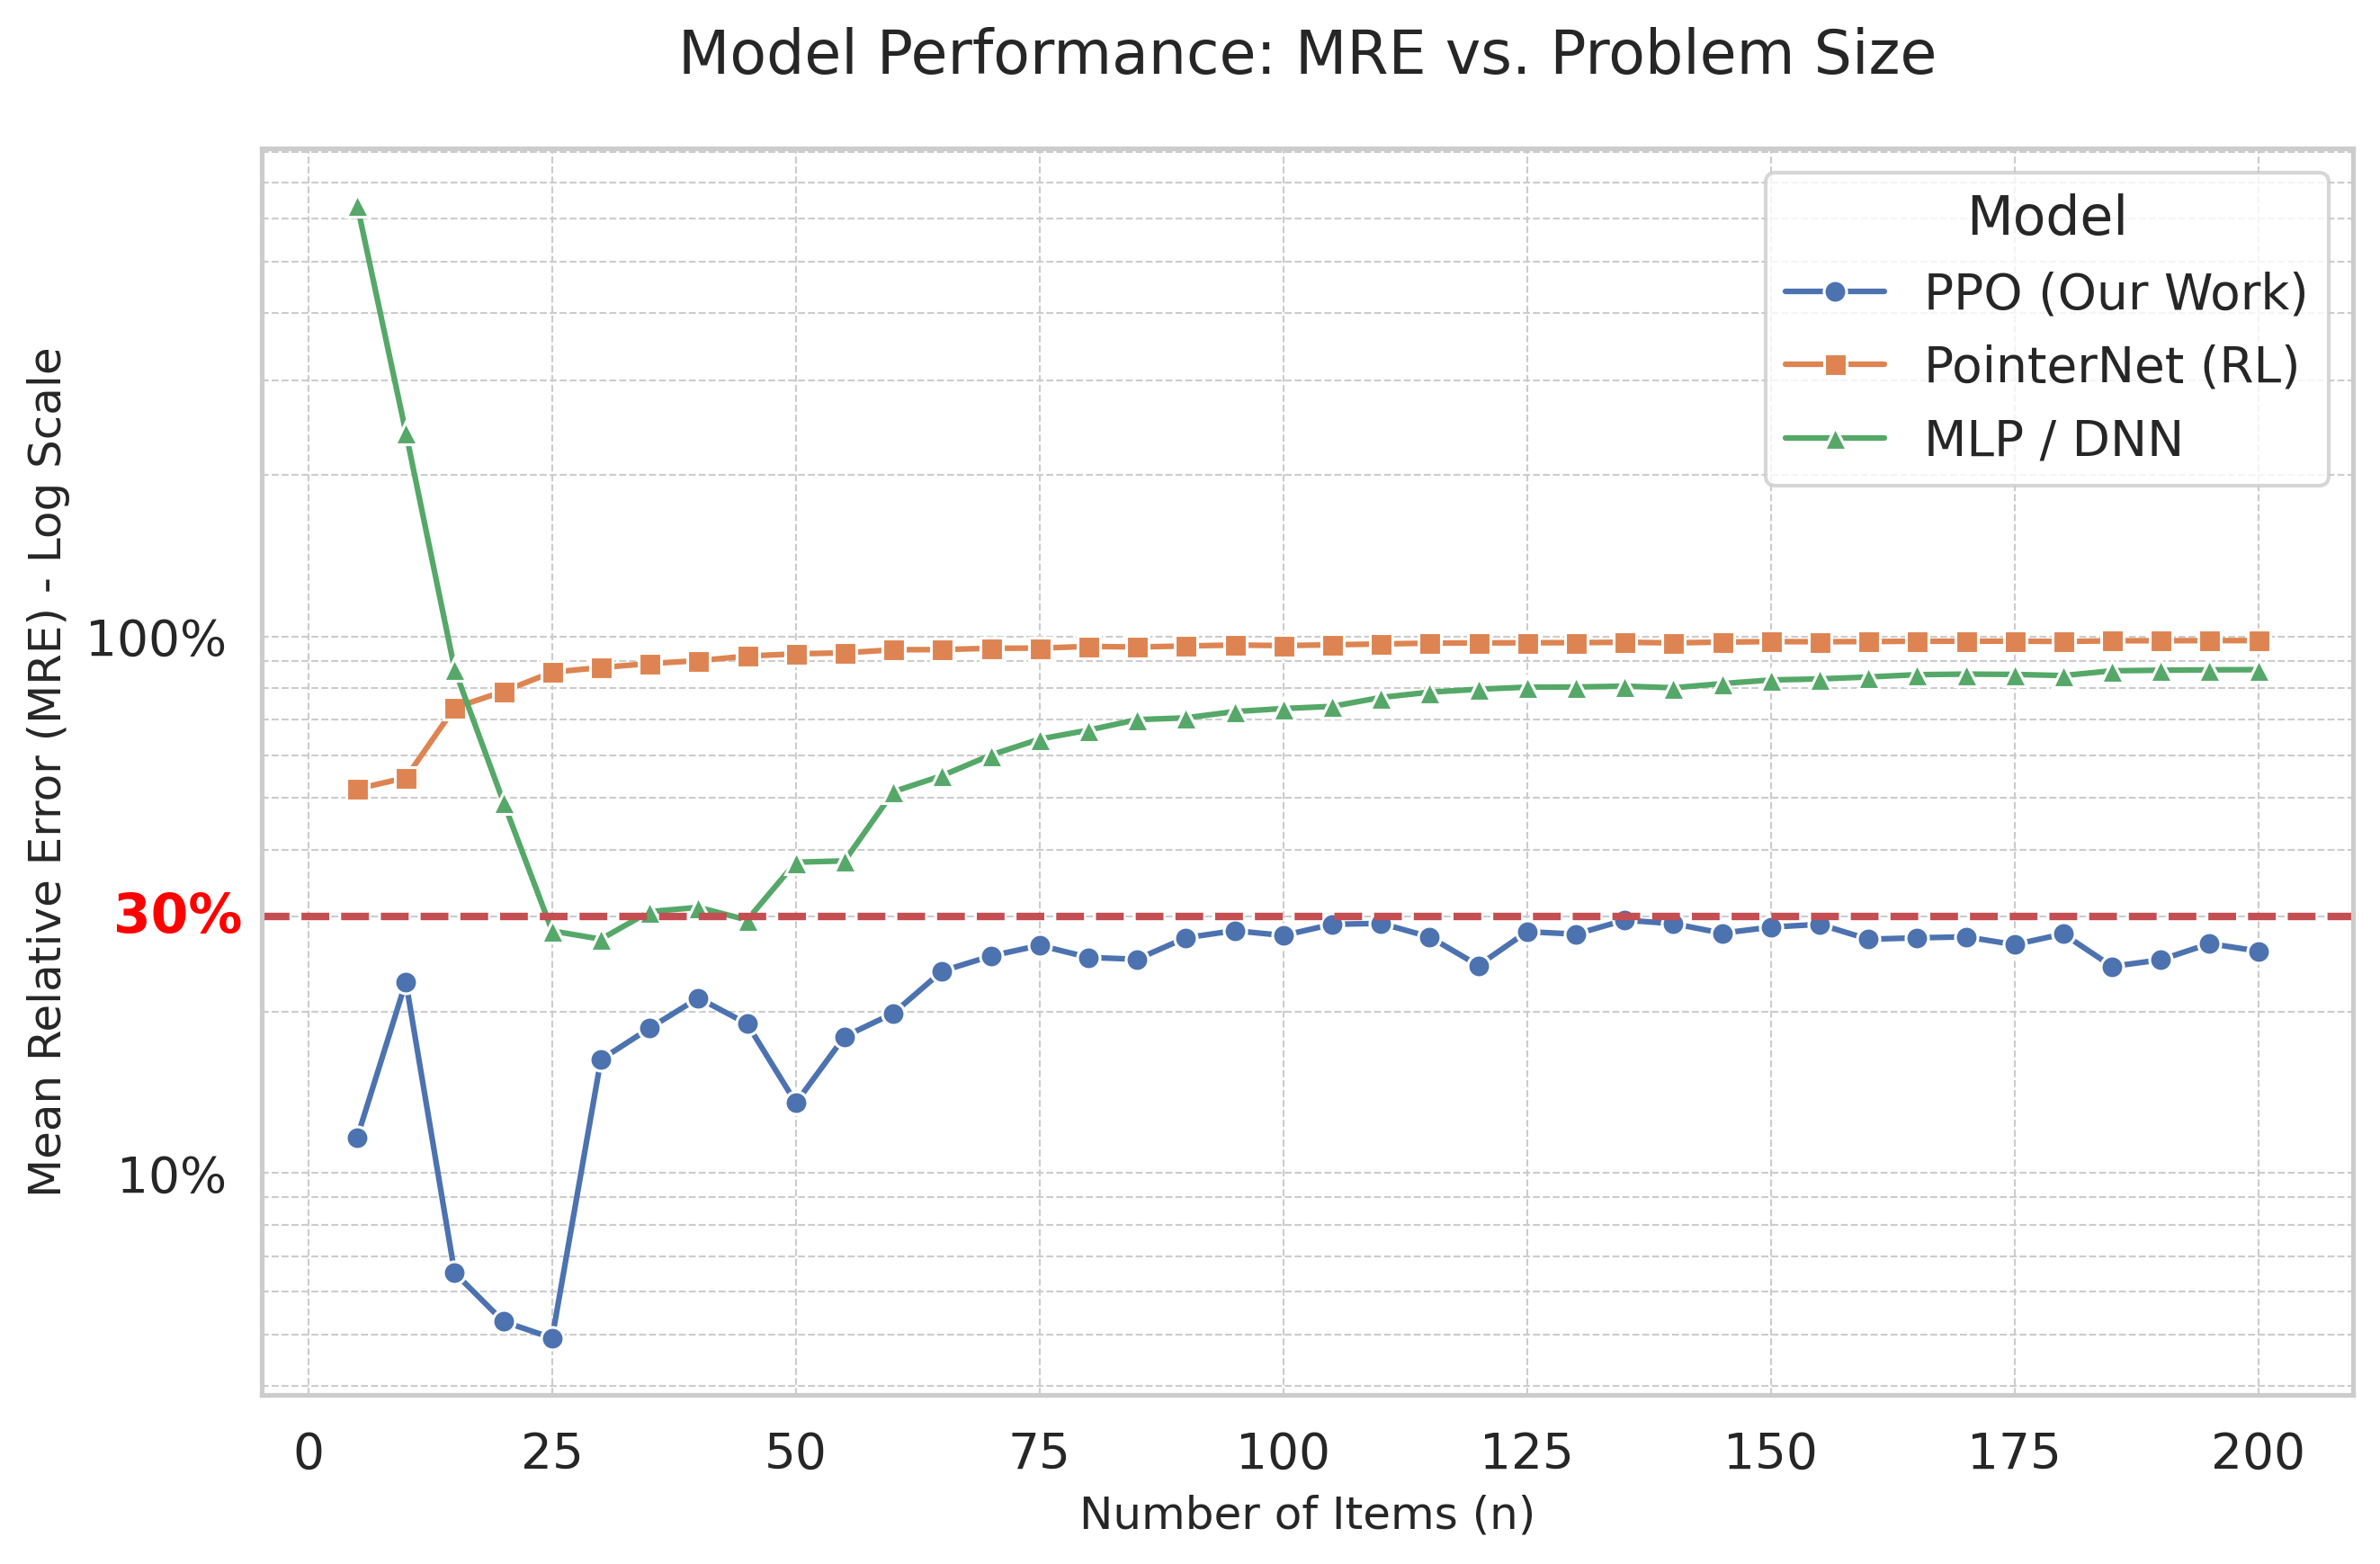
\includegraphics[width=0.48\textwidth]{mre_vs_problem_size_styled.png}
            \label{fig:mre_results}
        }
        \hfill % Creates a flexible space between the figures
        \subfloat[Inference Time vs. Problem Size.]{
            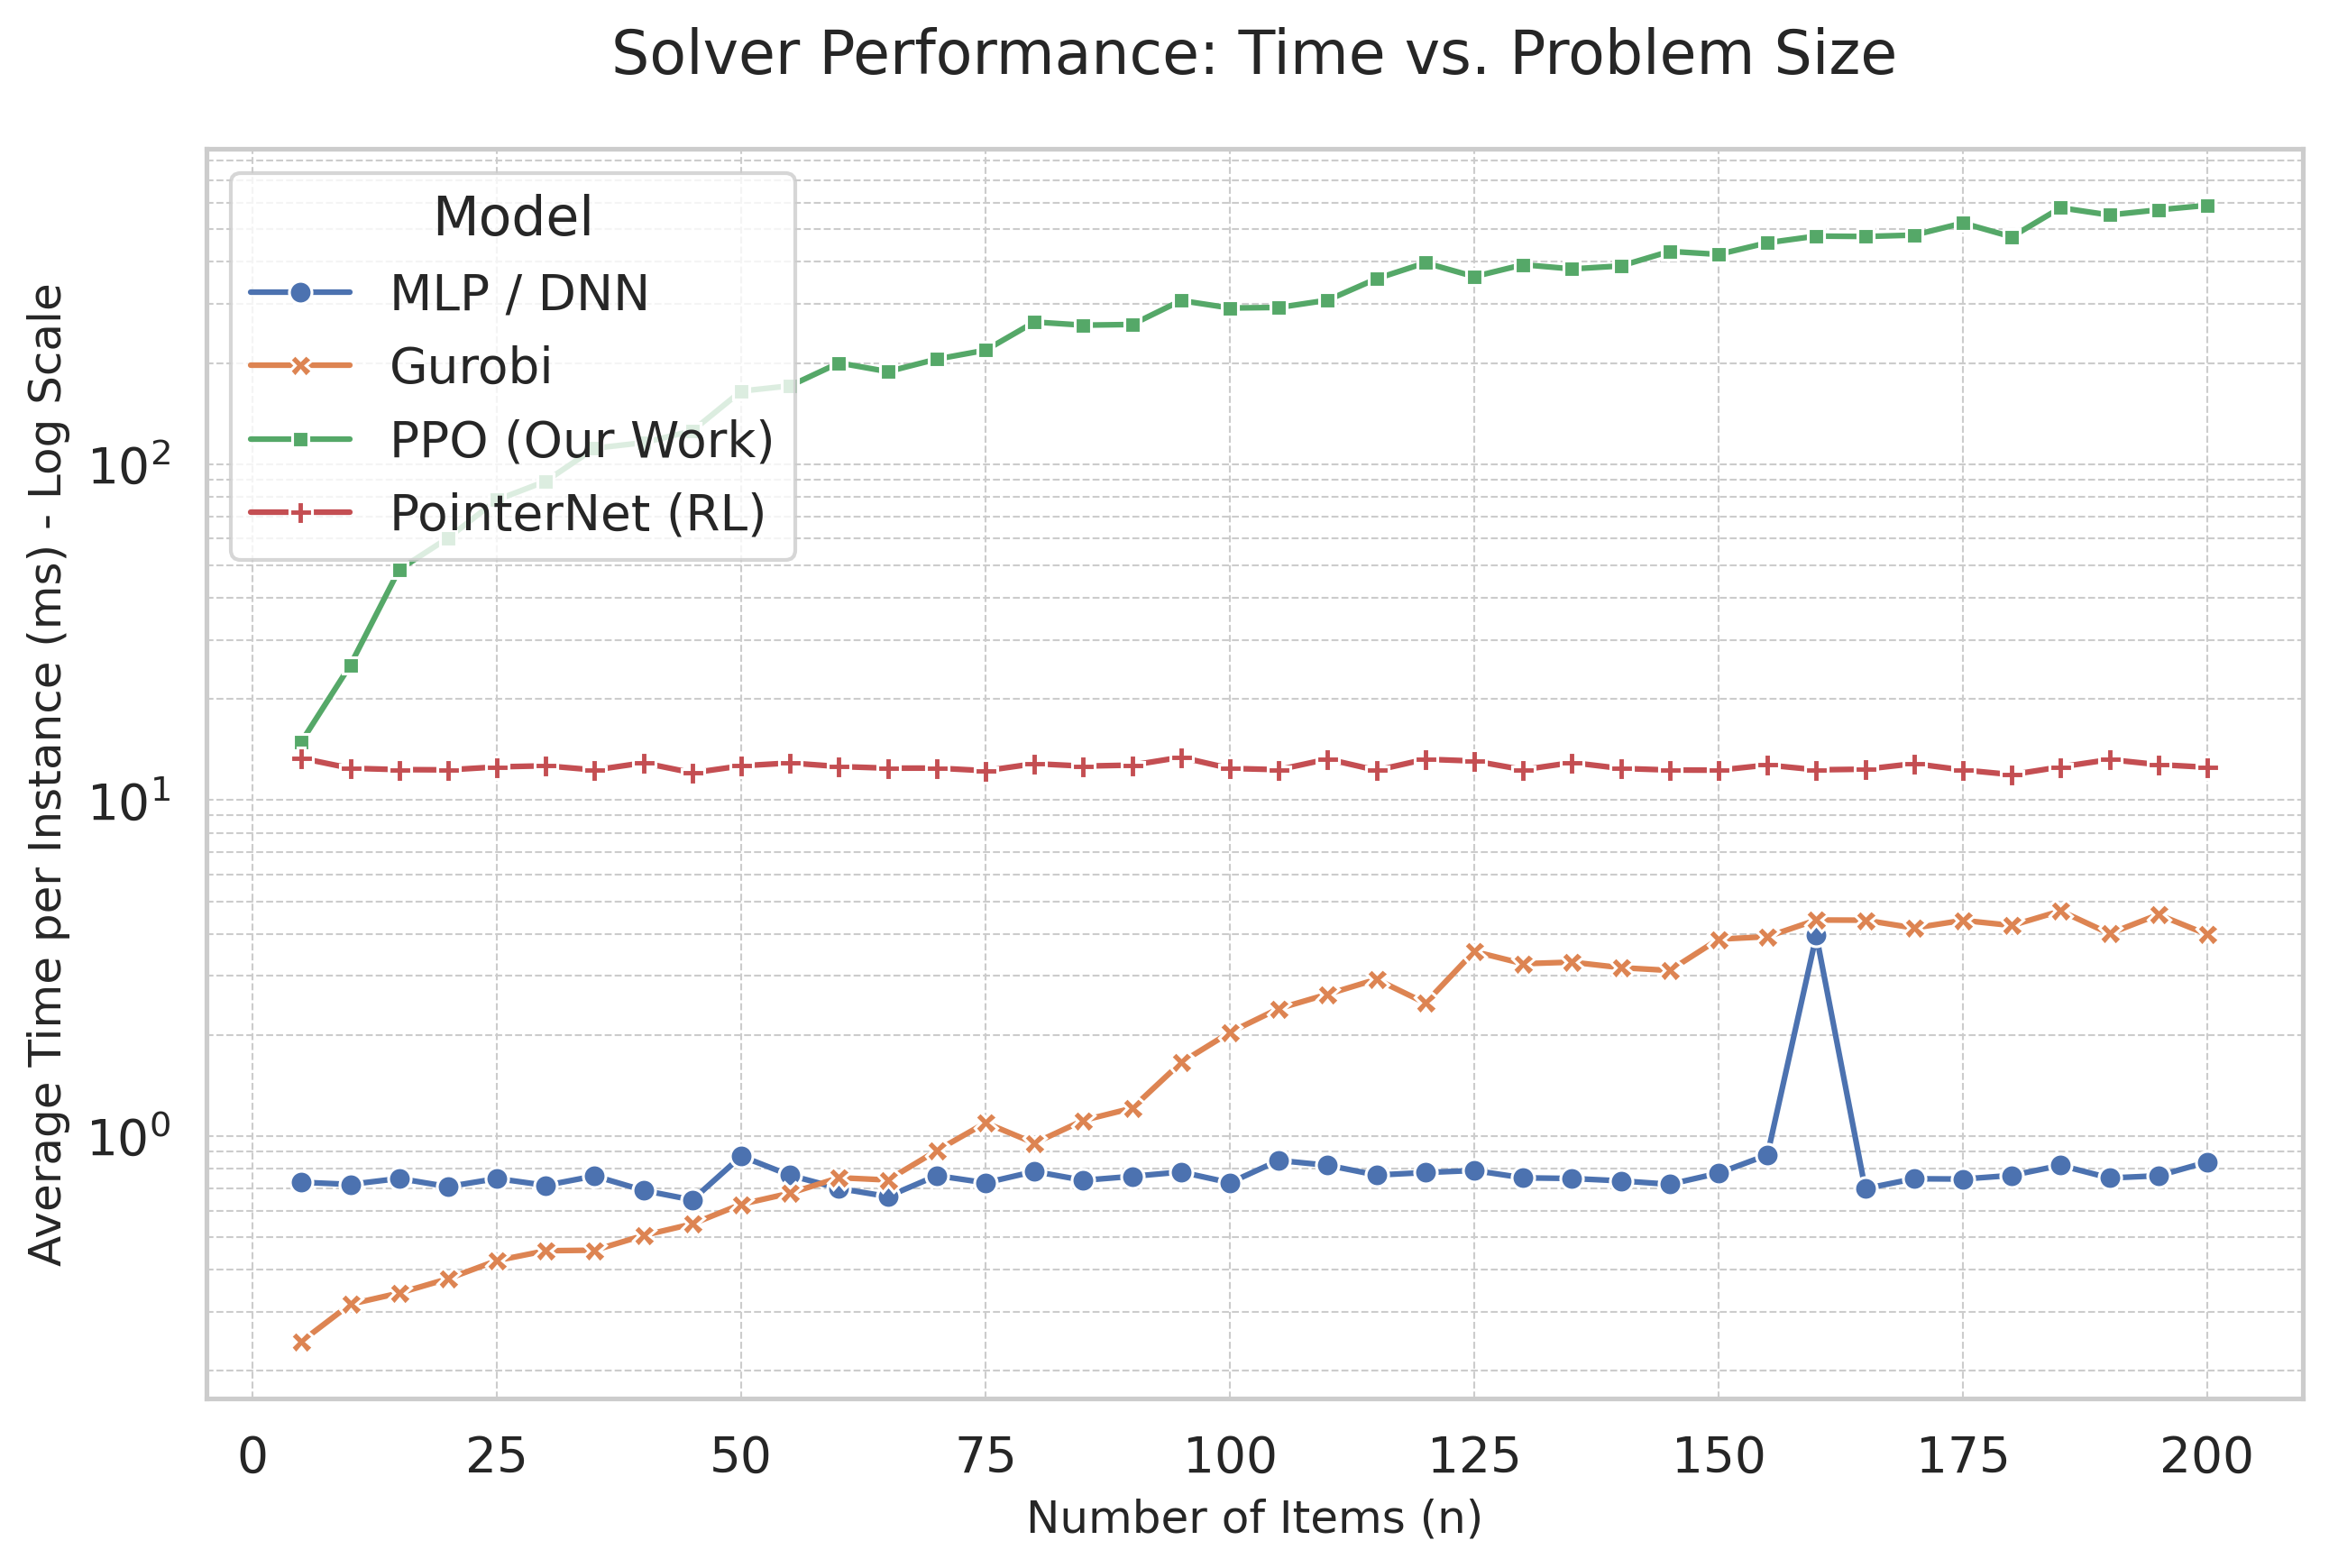
\includegraphics[width=0.48\textwidth]{evaluation_times_vs_n_styled.png}
            \label{fig:time_results}
        }
    \end{figure}
    
    \vspace{-0.6em} % Reduce the space between figures and the text below

    % --- BOTTOM PART: Analysis text in two columns ---
    \begin{columns}[T]
        % --- LEFT COLUMN: Analysis for the MRE plot ---
        \begin{column}{0.5\textwidth}
            \begin{block}{Key Findings: Accuracy}
                \begin{itemize}
                    \item Our PPO model maintains a low Mean Relative Error (MRE), demonstrating high solution quality and strong generalization.
                    \item Pointer Network shows a higher error rate.
                    \item The pure MLP model fails to generalize effectively.
                \end{itemize}
            \end{block}
        \end{column}

        % --- RIGHT COLUMN: Analysis for the Time plot ---
        \begin{column}{0.5\textwidth}
            \begin{block}{Key Findings: Inference Time}
                \begin{itemize}
                    \item PPO's inference time is practical for large instances.
                    \item Pointer Network is faster but less accurate.
                    \item MLP is the fastest but provides poor solutions.
                \end{itemize}
            \end{block}
        \end{column}
    \end{columns}
\end{frame}